\subsection{Hardware Details and Safety Features}\label{sec:HardwareDetails}\label{sec:SafetyFeatures}
CALIS offers various safety features to ensure that this device runs smoothly, that no components are lost inside the detector, that any detector contamination by dirty or incompatible materials is avoided, that pressure is maintained and that the introduction of oxygen or water into the LS and TMB is avoided. %, operation in the volume that excludes possibility of contact with PMTs or light pulsers (pacman) attached to each PMT.

\begin{description}

\item[Cable strength:]
The cables holding the deployment device are rated for loads over 1300\,lbs, while the device's weight is at the level of 20-30\,lbs, thus well below the cables' breaking strength.

\item[Drive mechanism:]
A magnetic brake, which releases only in the presence of electric power, ensures that the deployment device does not move, if a power failure occurs. Servo motor torque is limited in case of an unexpected load and the risk of breaking the cable is avoided.

The speed reducer is implemented in a double worm gear design. The primary worm gear has a 50:1 reduction and the secondary worm has an 82:1 reduction. The servo motor input speed is 2400 RPMs, the output is 0.6 RPM and its weight capacity is 148 lbs. If a power failure occurs, the speed reducer can hold the load at any position. The motor speed has been limited to 0.4\,cm/s, minimizing any lateral oscillation of the deployment device during lowering and raising of the source. This is also the maximum speed at which the motor does not overheat.

\item[Light and leak tightness of CALIS:]
When data is taken with the \lsv\ while the gate valve is open, as is the case during calibration campaigns with CALIS, absolute light tightness and pressure leak tightness is required. All view ports are covered with light tight covers when the gate valve is open. Both light and leak tightness was extensively validated throughout the manufacturing process, commissioning and during calibration campaigns.

\item[Securing source:] 
All connection points for the source and the source arm have been secured with two push locking pins that cannot be disengaged without a person pressing the pin. In addition, the source holder and its two locking pins are all tethered from outside the view port until they are locked in place, preventing them from accidentally falling into the interior of the CALIS housing.

\item[Manual retraction system:]
It is possible to manually retract the deployment device back to its home position and to close the gate valve in the unlikely event of a complete motor failure while the deployment device is deployed. The motor is disengaged, and a wrench is used to manually wind the cables back on the spools and to retract the deployment device above the gate valve. During this procedure, the nitrogen blanket protecting the \lsv\ is preserved. 
   
\item[High limit switch:]
A high limit switch is a hardware interlock that prevents the deployment device from hitting cable spools and gears, should it pass beyond the home position in the CALIS housing (Fig.~\ref{fig:CALISMechanism}). 
\end{description}

Thus far during calibration campaigns it has not been necessary to use the manual retraction system nor has the high limit switch been activated.
	
%%%%%%%%%%%%%%%%%%%%%%%%%%%%%%%%%%%%%%%%%
%%%%%%%%%%%%%%%%%%%%%%%%%%%%%%%%%%%%%%%%%

\subsection{Degrees of Freedom}

CALIS is capable of deploying sources at various positions inside the \lsv. Besides movement along $z$ down to its maximum cable length, it is possible to articulate at an angle $\theta$ between 0$^{\circ}$ and 90$^{\circ}$, where $\theta$ is the zenith-angle (Fig.~\ref{fig:DeploymentDevice}). Angles of more than 90$^{\circ}$ are excluded because the articulation chain's end is reached at a 90$^{\circ}$ angle (see photo inset in Fig.~\ref{fig:DeploymentDevice}).

\subsubsection*{$XY$-plane rotation}\label{sec:XYrotation}
The connection below the view port has an o-ring seal and uses a ring clamp to compress the seal. This clamp can be slightly loosened allowing the upper assembly (everything above and including the view port) to be rotated with respect to the lower assembly and the \tpc. Rotation in the $xy$-plane can even be performed while the device is deployed next to the cryostat, since the seal is helium leak and light tight even when loosened.

In principle a rotation by an arbitrary angle can be done, except when the arm would interfere with the cryostat. In one calibration campaign an \AmBe\ neutron source was deployed directly next to the cryostat and rotated away to an angle $\phi\,=\,90^\circ$.  A relative comparison between the two data sets as well as comparisons with Monte Carlo simulations gave insights on optical shadowing effects by the cryostat (Sec.~\ref{sec:CalibCampaigns}). 

%For articulation, there is currently a choice of three arm lengths---40.3\,cm,  57.15\,cm and 62\,cm.  
%Each of these lengths are measured from the center line of the organ pipe to the end of the source holder.  The arm lengths, 57.15\,cm and 62\,cm are intentionally made too long as they will be used to determine the exact location of the cryostat; some uncertainty in the cryostat's z and lateral position exist at the level of 3 - 4\,cm. The organ pipe we intend to use is 81\,cm distant from the cryostat center (and the geometric center of the LSV sphere) as measured from the center line of the organ pipe. The cryostat is 32\,cm in radius, which leaves a distance of $\sim$49\,cm to be reached  by the arm.


\begin{figure}[htbp]
 \centering
  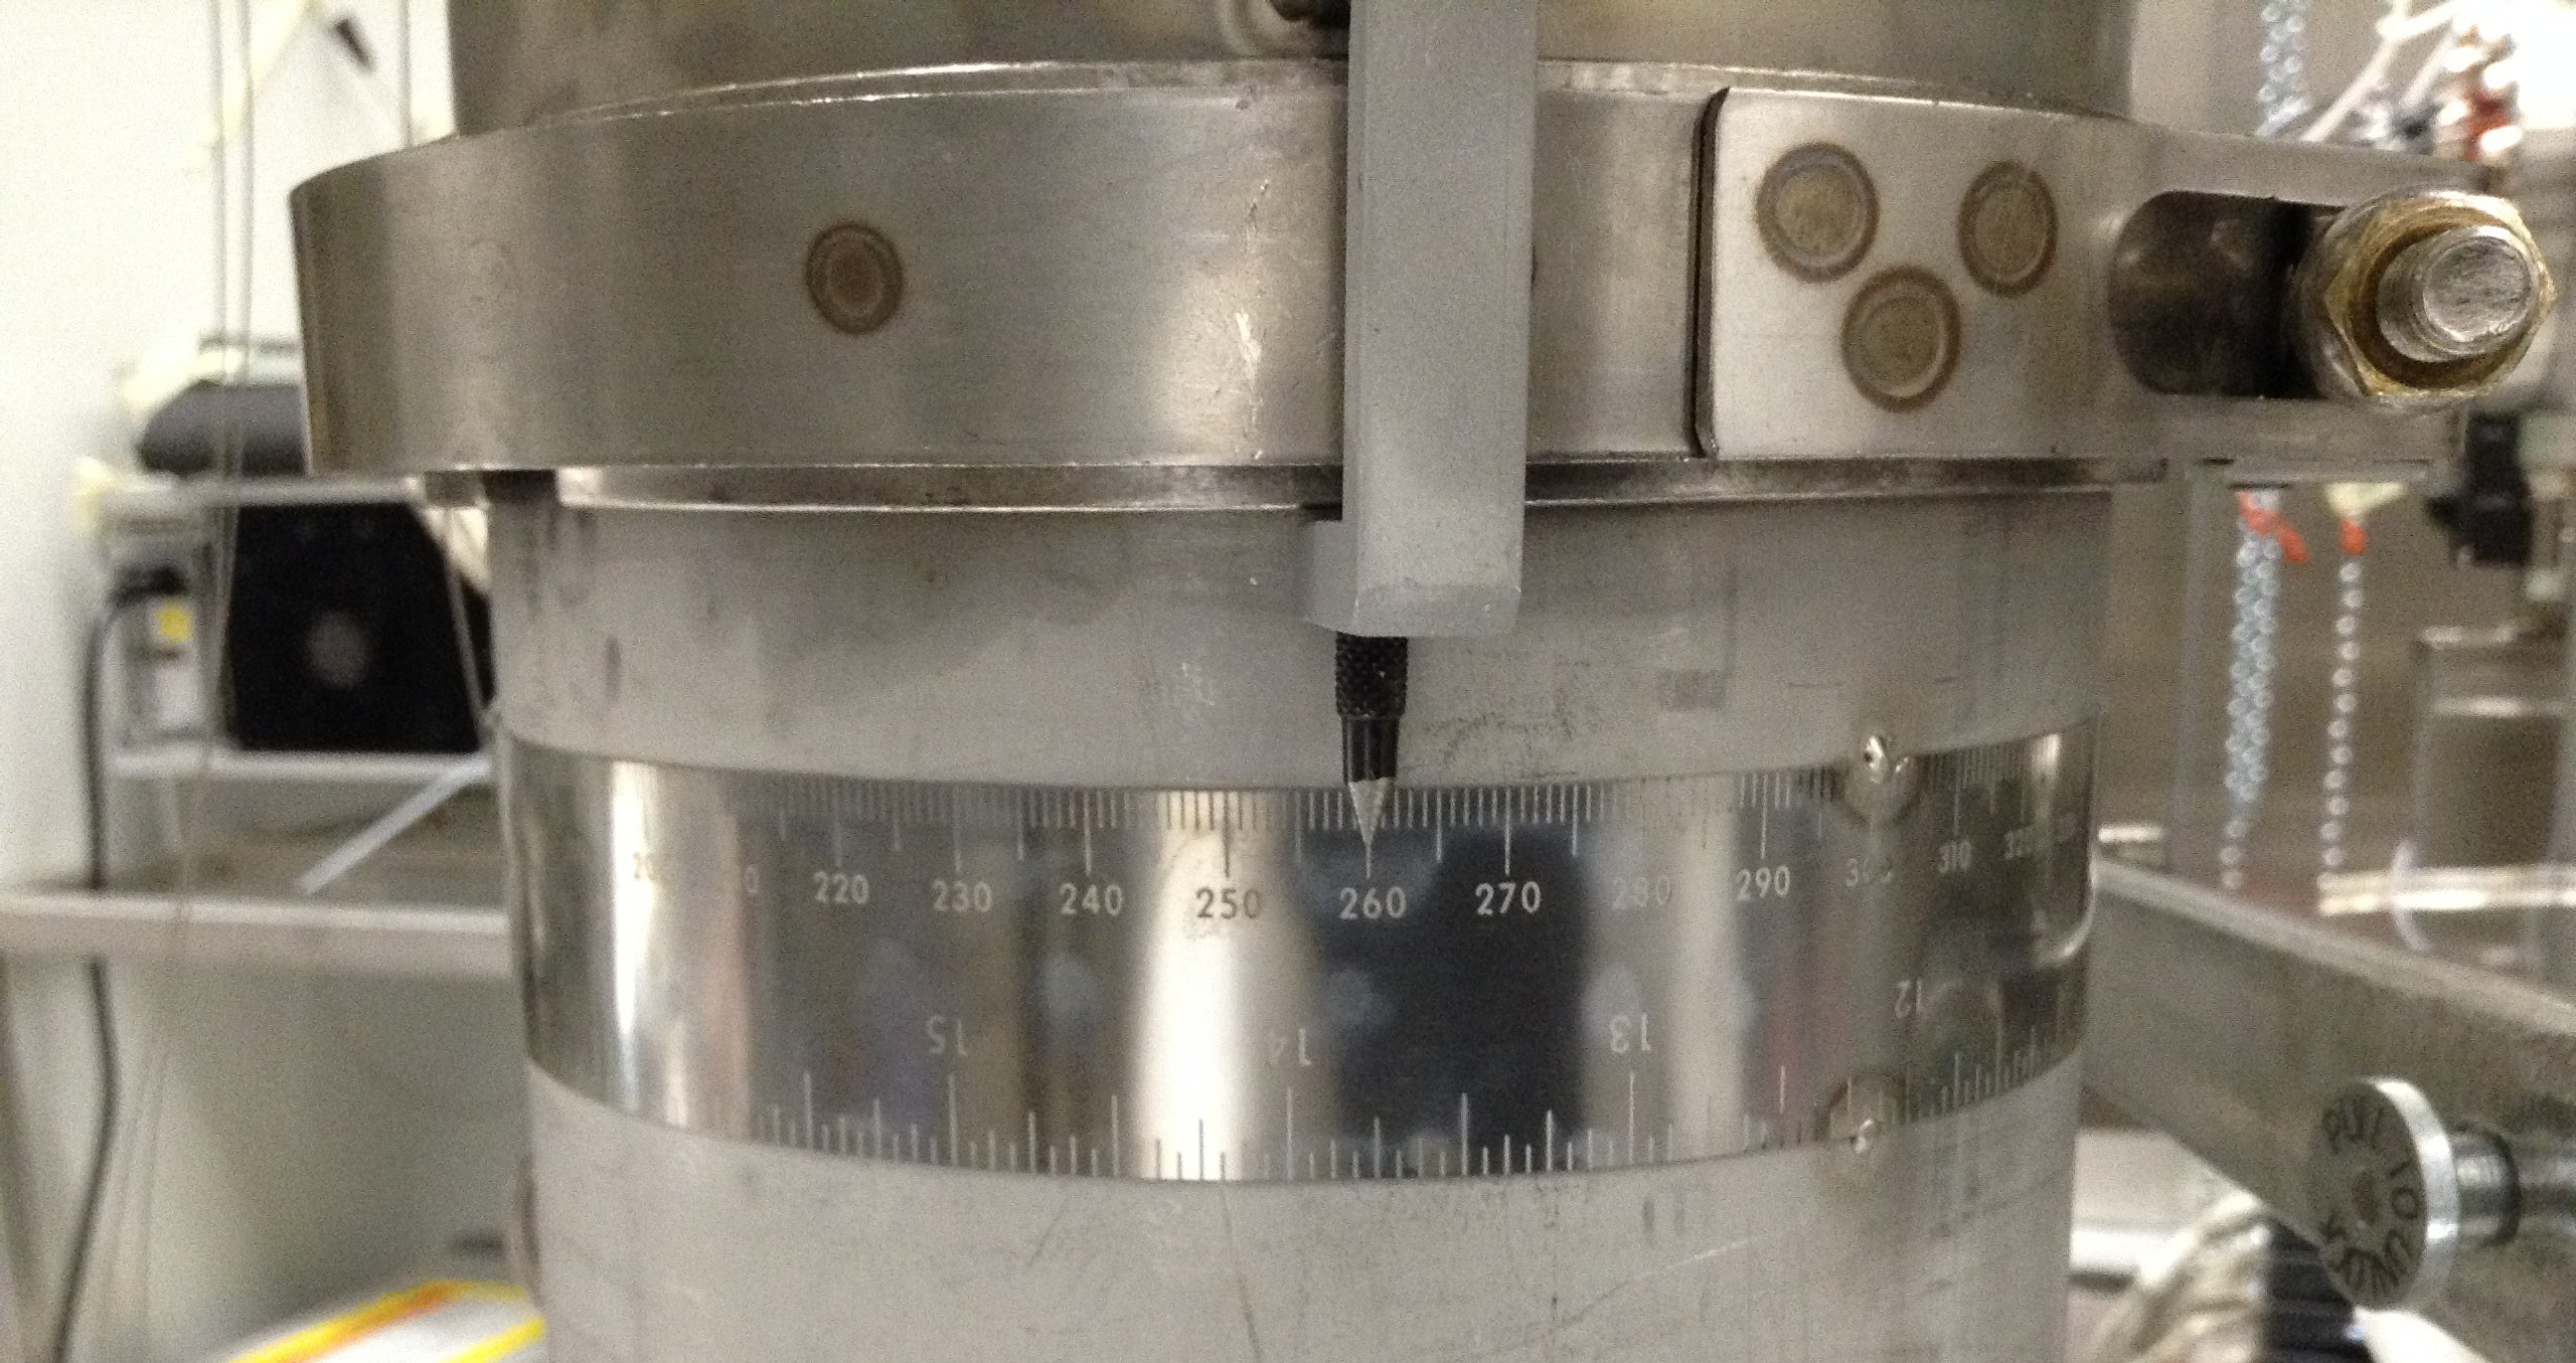
\includegraphics[width=0.7\textwidth]{Figures/RingClamp_WithPin_IMG_2669.JPG}
%  \includegraphics[scale=0.5]{Figures/RingClamp.jpg}
  \caption{Beneath the view port is a ring clamp with a ruler underneath. The rotation angle is read from the ruler going around the pipe. The ruler is in mm, which has been calibrated in degrees. To perform azimuthal rotation, the ring clamp is slightly loosened, and the entire upper assembly is rotated with respect to the lower assembly, along with the deployment device.}
  \label{fig:ring_clamp}
\end{figure} 

\subsubsection*{``No fly'' zone}
A ``no fly'' zone is defined directly above the cryostat where there are many TPC supply tubes. The source arm may not enter in this region, hence CALIS operators, who are specifically trained personnel to manipulate CALIS, are required to avoid articulation in this region. Since articulation is done manually and slowly by the operator, accidental entanglement of the source arm in the supply tubes is extremely unlikely.

%\begin{figure}[htbp]
% \centering
%  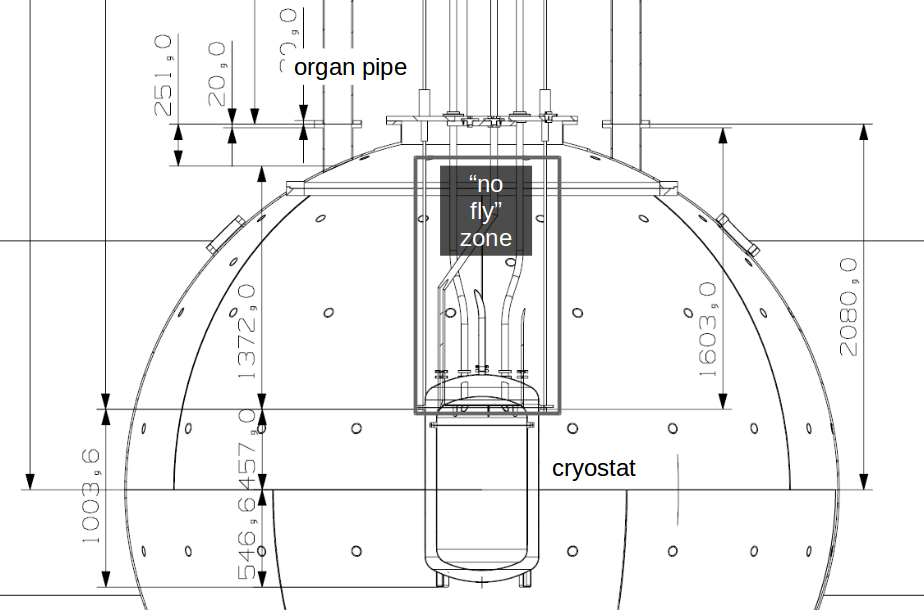
\includegraphics[scale=0.5]{Figures/NoFlyZone.png}
%  \caption{``No fly'' zone for the CALIS source arm.}
%  \label{fig:NoFlyZone}
%\end{figure} 

\subsubsection*{Default configuration}\label{sec:DefaultConfig}\label{sec:CentralPosition}
By default, the deployment device has been deployed with the longest source arm (62 cm) in a horizontal position in contact with the cryostat and to our 'central position' in $z$. The 'central position' is a motor step position, which we calibrated using $t_{drift}$ distributions of $^{133}$Ba to be within two centimeter of the TPC's active volume center (see Fig.~\ref{fig:SourcePosition}). 

Other degrees of freedom could involve shorter arm lengths, while longer arm lengths would require hardware modifications on the deployment device. Out of four organ pipes, a second one is available for source calibration. (Two organ pipes are not available due to interference with existing infrastructure: the cryogenic tower and the electronics rack.) Moving CALIS to a different organ pipe requires a partial disassembly of CALIS and reinstallation on the other organ pipe's gate valve.

%Finally CALIS is designed to house also a different deployment device, such as currently being planned for the neutron gun \cite{???}.